\documentclass[11pt]{article}
\usepackage[top=2cm, bottom=3.cm, left=2.5cm, right=2.5cm]{geometry}
\usepackage[utf8]{inputenc}
\usepackage{amsmath,amsthm,amsfonts,amssymb,amscd}
\usepackage{lastpage}
\usepackage{graphicx}
\usepackage{natbib}
\usepackage{hyperref}
\nonstopmode

\bibliographystyle{aasjournal}

\setlength{\parindent}{0.0in}
\setlength{\parskip}{0.05in}

\hypersetup{%
  colorlinks=true,
  linkcolor=blue,
  linkbordercolor={0 0 1},
  citecolor=blue,
  urlcolor=blue,
}

\newcommand{\code}{\texttt}

\begin{document}

\title{\textbf{Charting the Growth of Galaxies} \\[0.25cm] \large{CTA200H | 2020 Summer}}
\author{Jeff Shen \\ Advisor: Dr. Allison Man}
\date{\today}
\maketitle

% problem 1
\section*{Spectral Fitting}

We begin with Fig. \ref{fig:initial_spectra} of the three multiple images of galaxy 2 (Gal. 2a, 2b, and 2c) as defined in \cite{MacKenzie2014}. The first spectrum, for Gal. 2a, appears to be entirely noise, as there is no distinct peak like there is for the other two spectra. In the second and third panels of the figure, there are peaks in the intensity at around 88 GHz. 

\begin{figure}[!htbp]
    \centering
    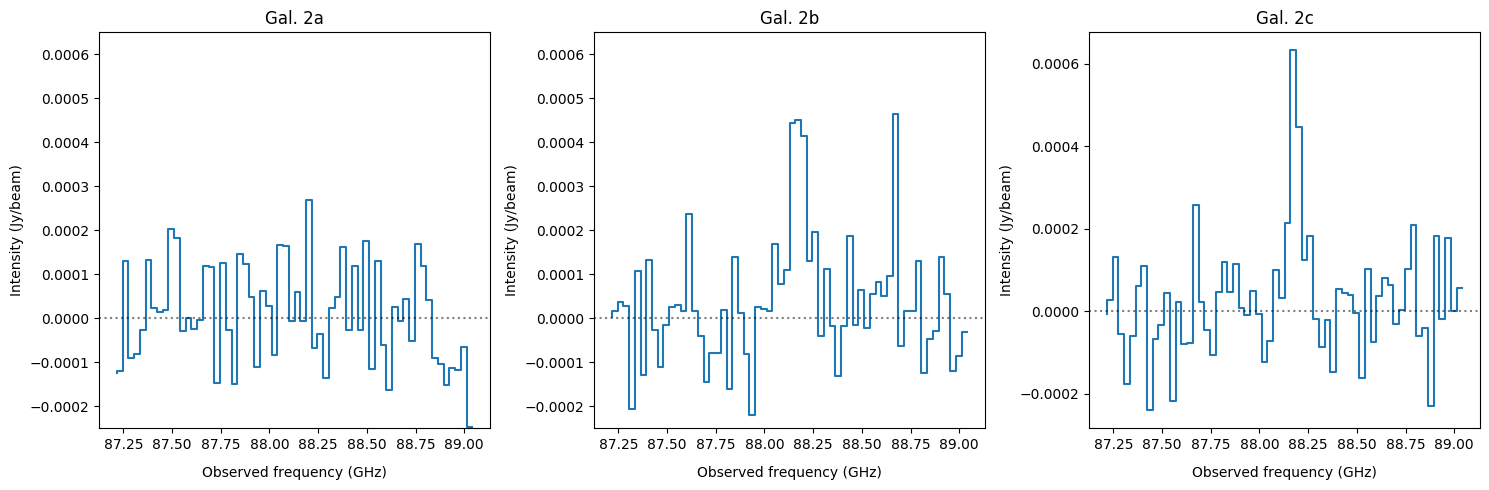
\includegraphics[width=\linewidth]{../figs/initial_spectra.png}
	\caption{Plot of the extracted spectra of the multiple images of Gal. 2. Observed frequency (GHz) is plotted against the intensity (Jy/beam).}
    \label{fig:initial_spectra}
\end{figure}

The Levenberg–Marquardt algorithm\footnote{https://en.wikipedia.org/wiki/Levenberg-Marquardt\_algorithm} from \code{astropy.modeling}, which minimizes the sum of squared residuals (SSR), was used to fit a 1D Gaussian model to each of the spectra. The results are shown in Fig. \ref{fig:gaussian_fit}. As expected, the algorithm had some trouble identifying a distinct peak for Gal. 2a, and as a result, the fitted Gaussian line for that image is much broader and has a smaller amplitude than the lines for the other two images.

The peak observed frequencies can be found in Table \ref{table:peaks_zs}, along with the full width at half maximum (FWHM) for each fit. For a Gaussian, the FWHM can be calculated\footnote{https://mathworld.wolfram.com/GaussianFunction.html} from the standard deviation $\sigma$ as 
\begin{align*}
	\rm{FWHM} = 2\sqrt{2\log{2}}\sigma.
\end{align*}

\begin{figure}[!htbp]
    \centering
    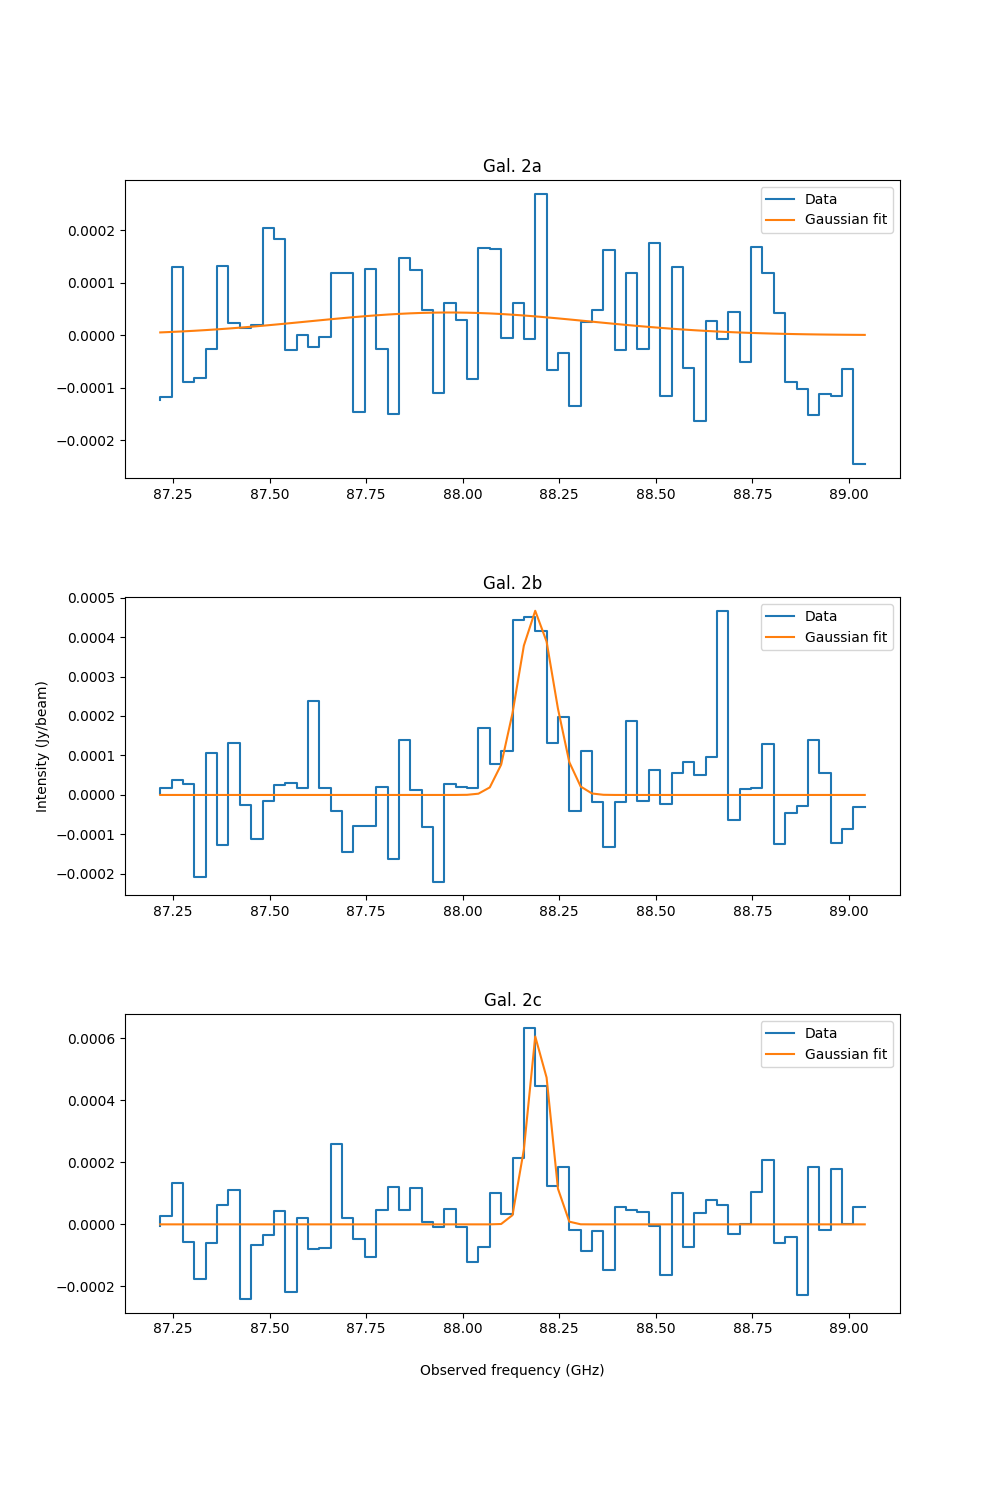
\includegraphics[width=0.8\linewidth]{../figs/gaussian_fit.png}
    \caption{Plot of the spectra of each lensed image, with a 1D Gaussian fit in orange. There are distinct peaks for the spectra of Gal. 2b and 2c.}
    \label{fig:gaussian_fit}
\end{figure}

Spectroscopic redshift can be calculated for an object using the formula 
\begin{align*}
	z = \frac{v}{v_0} - 1,
\end{align*}
where $v$ is the observed frequency and $v_0$ is the rest-frame frequency. In thie case, the target transition in these spectra is the $^{12}$CO(J=3-2) transition, which has a rest-frame frequency of 345.8 GHz \citep{Carilli2013}. The observed frequency for each of the images was taken to be the mean of the Gaussian fit. The results are given in Table \ref{table:peaks_zs}, and they are in line with what is expected (see. Table 1 in \cite{MacKenzie2014}).

Using the calculated spectroscopic redshift, it is possible to convert the observed frequencies into radio velocities. First, the rest frequency of the $^{12}$CO(J=3-2) transition is shifted so velocities are relative to a redshift (ie. the source has zero velocity):
\begin{align*}
	v_s = \frac{v_0}{z+1},
\end{align*}
where $v_s$ is the shifted rest frequency, $v_0$ is the unshifted rest frequency, and $z$ is the redshift of the source. Then, the radio velocity is given by 
\begin{align*}
	V_{rad} = (1 - \frac{v}{v_s})c,
\end{align*}
where $V_{rad}$ is the radio velocity, $v$ and $v_s$ are defined as before, and $c$ is the speed of light. 

For each of the galaxies, the root mean square (RMS) of the intensity of the spectrum was calculated. This was done in order to better understand whether those detections are merely noise or not. For the spectra of Gal. 2b and 2c, the line detections were masked out, and the calculation was done on the rest of the data. The equation for RMS, given $n$ data points $x_1, \ldots, x_n$, is 

\begin{align*}
	\rm{RMS} = \sqrt{\frac{1}{n}\sum_i^nx_i^2}.
\end{align*}

\begin{figure}[!htbp]
    \centering
    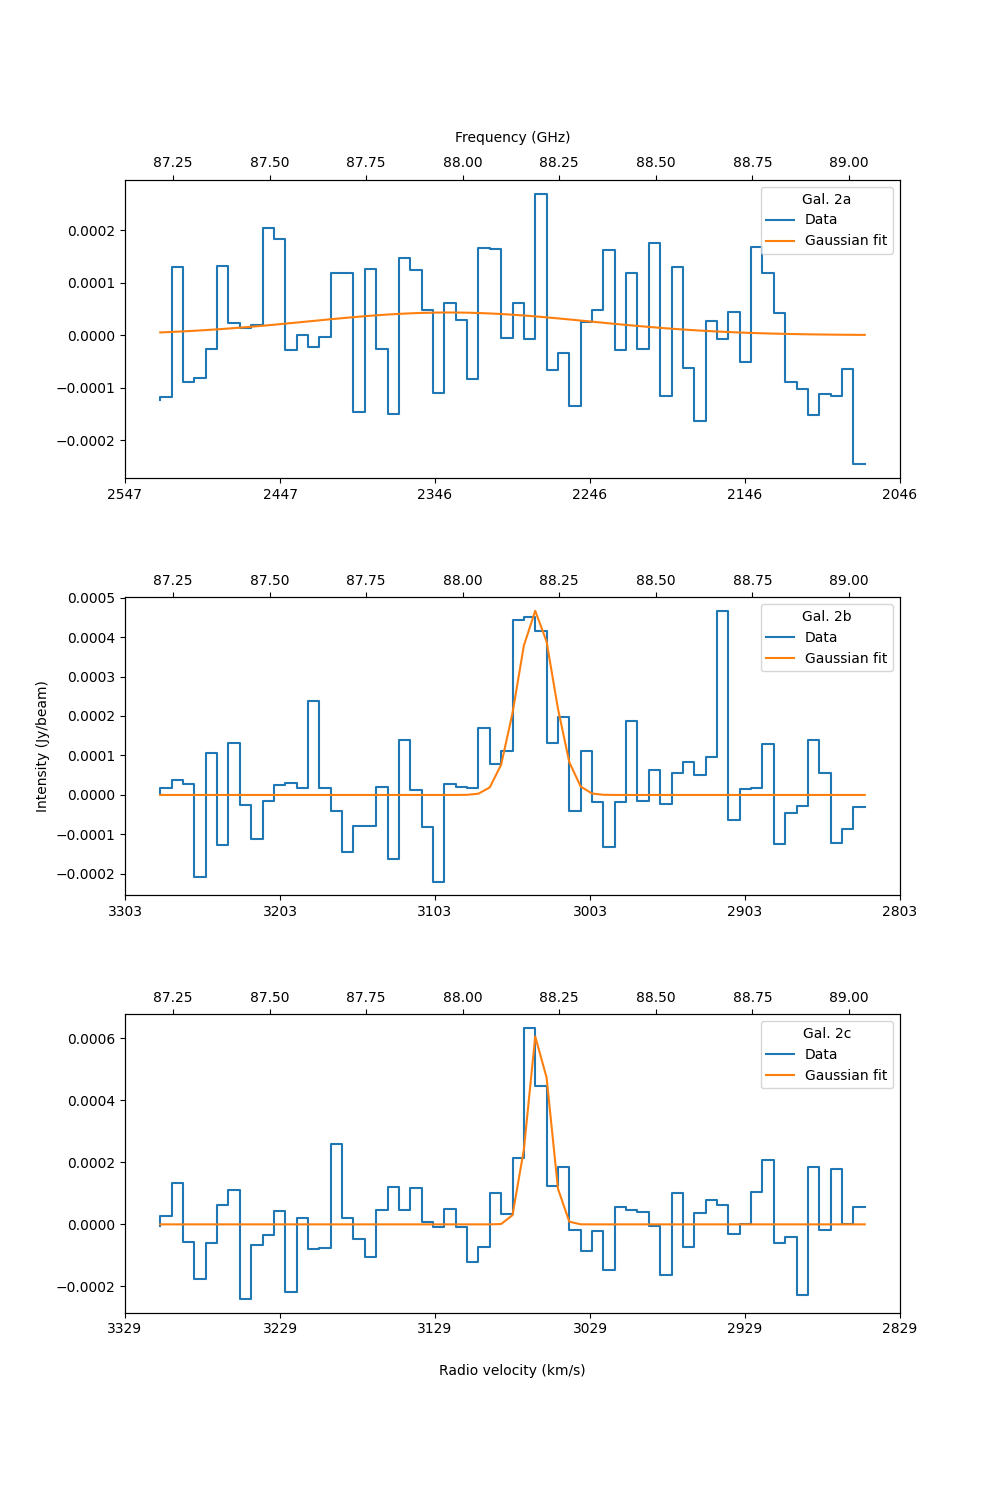
\includegraphics[width=0.8\linewidth]{../figs/redshift_axis_plot.png}
	\caption{Plot of the spectra with a 1D Gaussian fit (same as Fig \ref{fig:gaussian_fit}). Bottom x-axis is in radio velocity (km/s) with reference to the redshift to each image. Top x-axis is in observed frequency (GHz). y-axis is in intensity (Jy/beam). Note that the radio velocity increases going to the left, whereas the frequency increases going to the right.}
    \label{fig:redshift_axis}
\end{figure}

\begin{table}[!htbp]
\centering
\begin{tabular}{ccccc}
\hline \\[-0.25cm]
Gal & Peak Observed Frequency & Line Width & RMSE & Redshift \\
ID  & GHz                     & FWHM       &      & \\[0.1cm]
\hline \\[-0.25cm]
2a & 87.96 & 0.858 & 1.11E-04 & 2.93\\
2b & 88.19 & 0.111 & 1.15E-04 & 2.92\\
2c & 88.20 & 0.064 & 1.08E-04 & 2.92\\
\hline
\end{tabular}
\caption{Mean of the Gaussian fit, FWHM line width, RMS error, and redshift for each of the lensed images of Gal. 2.}
\label{table:peaks_zs}
\end{table}

% problem 2
\section*{Measuring Line Luminosity}

\begin{table}[!htbp]
\centering
\begin{tabular}{cccc}
\hline \\[-0.25cm]
Gal & $S_{CO(3-2)}\Delta v$ & $D_L$ & $L'_{CO(3-2)}$ \\
ID  & $\rm{Jy\,km\,s^{-1}}$ & Mpc   & $\rm{K\,km\,s^{-1}\,pc^2}$ \\[0.1cm]
\hline \\[-0.25cm]
2a & $3.86\times 10^{-5}$ & $2.47\times 10^{4}$ & $1.63\times 10^{6}$ \\
2b & $5.49\times 10^{-5}$ & $2.46\times 10^{4}$ & $2.31\times 10^{6}$ \\
2c & $4.36\times 10^{-5}$ & $2.46\times 10^{4}$ & $1.83\times 10^{6}$ \\
\hline
\end{tabular}
\caption{Table to test captions and labels}
\label{table:2}
\end{table}

\section*{Measuring Gas Mass}

\begin{table}[!htbp]
\centering
\begin{tabular}{cccc}
\hline \\[-0.25cm]
Gal & $L'_{CO(1-0)}$             & $M_{gas}$ & Delensed $M_{gas}$ \\
ID  & $\rm{K\,km\,s^{-1}\,pc^2}$ & $M_\odot$ & $M_\odot$          \\[0.1cm]
\hline \\[-0.25cm]
2a & $6.05\times 10^{6}$ & $2.78\times 10^{7}$ & $9.73\times 10^{6}$ \\
2b & $8.55\times 10^{6}$ & $3.93\times 10^{7}$ & $4.86\times 10^{6}$ \\
2c & $6.79\times 10^{6}$ & $3.13\times 10^{7}$ & $5.12\times 10^{6}$ \\
\hline
\end{tabular}
\caption{Table to test captions and labels}
\label{table:3}
\end{table}

\begin{align*}
    \frac{|M_{2b} - M_{2c}|}{\frac{M_{2b}+M_{2c}}{2}} = \frac{2.6\times 10^{5}}{4.99\times 10^{6}} \simeq 5\%
\end{align*}

\section*{Wrapping Up}

\begin{figure}[!htbp]
    \hspace{-1cm}
    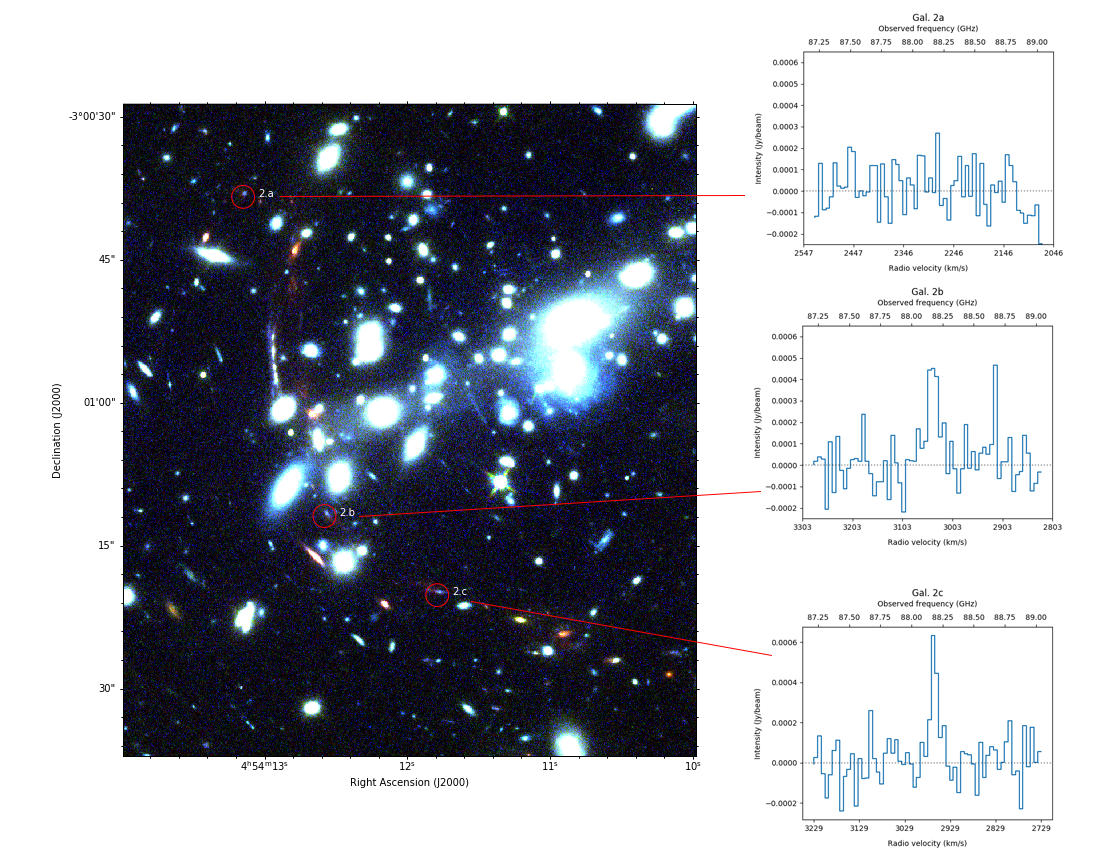
\includegraphics[width=1.1\linewidth]{../figs/final.png}
    \caption{RGB composite of MS 0451.6−0305 with F160W, F110W, and F814W filters, respectively. Multiple lensed images of Gal. 2 indicated. Spectra extracted from circles with a diameter of 1\". Bottom axes of spectra labelled in radio velocity relative to the redshift calculated for each image as in Table \ref{table:1}. Top axes in observed frequency (GHz). Side axes in intensity (Jy/beam).}
    \label{fig:final_oteo}
\end{figure}

\begin{table}[!htbp]
\centering
\begin{tabular}{cccc}
\hline \\[-0.25cm]
Gal & SFE \\
ID  & $\rm{yr^{-1}}$ \\[0.1cm]
\hline \\[-0.25cm]
2a & $1.02\times 10^{5}$ \\
2b & $2.04\times 10^{5}$ \\
2c & $1.93\times 10^{5}$ \\
\hline
\end{tabular}
\caption{Table to test captions and labels}
\label{table:4}
\end{table}

\nocite{*}
\bibliography{sources}

\end{document}

